
\begin{frame}{El SIOSE}
\begin{itemize}
\item El SIOSE es una valiosa \textbf{base de datos de ocupación del suelo} que contiene un gran volumen de información territorial de toda España.
\item Desde su aparición en 2005, SIOSE se ha convertido en un repositorio de referencia para sus homólogos europeos, llegando a ser un \textbf{modelo para la iniciativa EAGLE} (\textit{SIOSE europeo}). 
\item A pesar de su gran potencial, el SIOSE presenta ciertos problemas de \textit{usabilidad} debidos a su gran volumen y complejidad.
\end{itemize}
\end{frame}

\begin{frame}{El SIOSE}
\begin{figure}
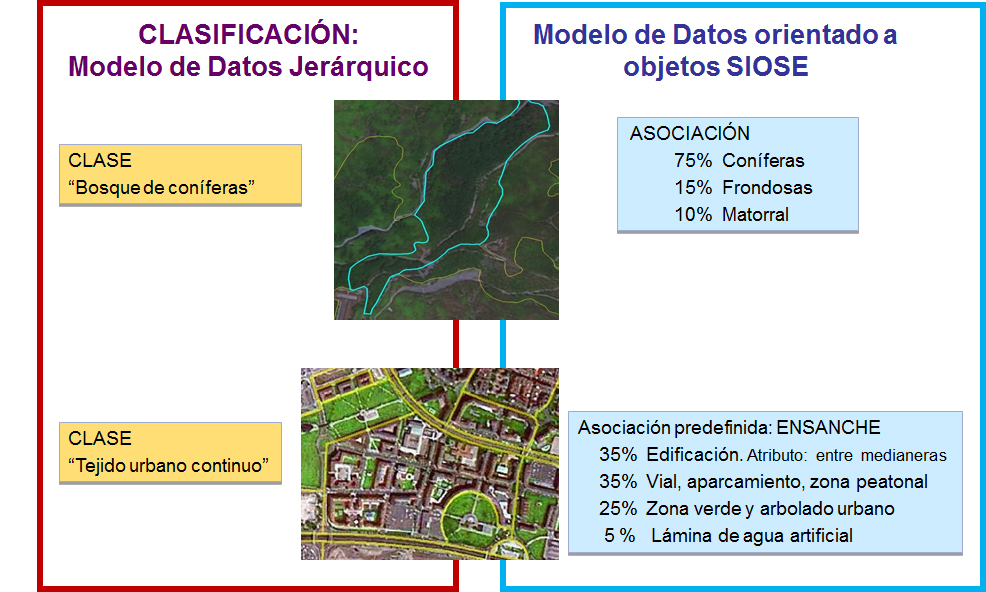
\includegraphics[height=5cm]{Introduccion/Figs/siose-oo.png}
%\caption{Riqueza descriptiva del modelo de datos orientado a objetos del SIOSE frente a una clasificación jerárquica. Fuente: \url{www.siose.es}.\label{fig:siose-oo}}
\end{figure}
\end{frame}

\begin{frame}{Métricas del paisaje}
\begin{itemize}
\item Las \textbf{métricas de paisaje} son métodos cuantitativos que sirven para analizar la estructura del paisaje y otros fenómenos (p.ej. evolución del paisaje, conectividad de ecosistemas, entre otros).
\item FRAGSTATS, Conefor Sensinode, Patch Analyst, entre otros, son aplicaciones de escritorio muy utilizadas para el cálculo de métricas del paisaje. No obstante, \textbf{no hay ninguna aplicación} que sea fácilmente \textbf{escalable y extensible} como para realizar análisis sobre una geodatabase similar a la del SIOSE.
\end{itemize}
\end{frame}


